\documentclass{llncs}
\usepackage{graphicx}
\begin{document}
\title{LITERATURE SURVEY ON THE BIN PACKING PROBLEM}
\author{MARTIN RAMALINGUM}
\institute{DURHAM UNIVERSITY}
\maketitle            
\section{KEY TERMS}
\subsection{2D Irregular Bin Packing Problem}
The two dimensional irregular bin packing problem (2DIBPP) is an NP-Hard combinatorial optimisation problem \cite{pandey2021analysis}. The aim is to allocate n irregular polygon pieces into N identical rectangular bins, minimising the number of bins used. The problem is defined formally as follows \cite{guerriero2022hierarchical}: 

Let P = \( p_1, p_2, ... p_n \) denote the set of irregular pieces. 
\mbox{Each piece \(p_k, k = 1, … n\)} is a polygon of area \(a_k\). 

Let B = \( b_1, b_2, ... b_N \) denote the set of N identical rectangular bins, where each bin has a fixed length of L and a fixed width of W. 
\\
The aim of the problem is to fit the n pieces into the fewest number of bins possible. It is assumed that all n pieces can fit into the N bins. \\
The following rules must also be obeyed in this variation of the problem:
\begin{itemize}
    \item Rotation of pieces is forbidden.
    \item Flipping (reflection) of pieces is forbidden.
    \item All pieces must be convex.
    \item Pieces cannot overlap with other pieces.
    \item Pieces must fit entirely within the bin.
\end{itemize}

A naive approach to evaluating the success of a solution to the problem would be to count the number of bins used. However, if two solutions used the same number of bins, simply counting the number of bins used would not be sufficient to compare them. Therefore, two functions are used to determine the success of a solution, the Fitness Function F used by Lopez-Camacho et al. \cite{lopez2014unified}, and the parameter K used in Martinez-Sykora et al \cite{martinez2017matheuristics}.

\subsection{Heuristics}
Heuristics aim to produce reasonable approximate solutions to a problem within a reasonable time, and are therefore highly applicable to NP-Hard optimisation problems within vast search spaces of solutions.

Hyper-heuristics, as defined by Burke et al. are \emph{“concerned with intelligently choosing the right heuristic or algorithm in a given situation”}\cite{burke2003hyper}. Hyper-heuristics search the space of lower-level heuristics and use a combination of them to try to outperform single statistics. Guerriero and Saccomanno \cite{guerriero2022hierarchical}, use a dynamic hierarchical hyper heuristic approach. ‘Dynamic’ refers to the fact that the low-level heuristics (selection, placement, and filling operators) can be chosen based on the particular instance of the problem. ‘Hierarchical’ refers to the structure of the main hyper-heuristic, being able to either use low-level heuristics or execute itself recursively (Fig 1). \\

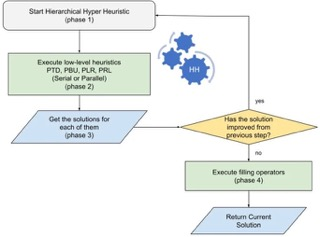
\includegraphics{hierarchical.jpeg} \\
\caption{Fig 1: The Hierarchical Heuristic scheme developed by Guerriero and Saccomanno.}


\section{CORE THEMES}


\subsection{Low-Level Heuristics (Operators)}
\subsection{Hierarchical Hyper Heuristics and Genetic Algorithms}
\subsection{Evaluating Solution Fitness}
Metrics are used to both guide the hyper-heuristics, especially when choosing filling operators, and to evaluate the success of the solution generated. The Fitness Function \emph{F} \cite{lopez2014unified}, is used by Guerriero et al. 
\subsection{Bin Packing Problem Variations}

\section{CONCLUSIONS}

\bibliographystyle{plain}
\bibliography{mybib}

\end{document}
